\section*{Results}
\label{results}

To find out how many time the stochastic transitivities is violated, each of the three types is investigated and the number of times there is a violation is counted. The results is shown in \autoref{tab:Stocha}. 

%Weak stochastic transitivity (WST) = 2 violations

%\noindent Moderate stochastic transitivity (MST) = 3 violations
 
%\noindent Strong stochastic transitivity (SST) = 25 violations

\begin{table}[H]
\centering
\begin{tabular}{@{}ll@{}}
\toprule
Stochastic transitivity     & Violations \\ \midrule
WST      & 2   \\
MST      & 3   \\
SST      & 25   \\ \bottomrule
\end{tabular}
\caption{Results for the number of violations of the three Stochastic transitivities.}
\label{tab:Stocha}
\end{table} 

\noindent To check how good a fit the BTL-model\fxnote{er det rigtigt?} is, a Chi-square test in conducted and the results is shown in \autoref{tab:Chi}. 

\begin{table}[H]
\centering
\begin{tabular}{@{}lll@{}}
\toprule
$\chi^{2}$     & Df & p-value \\ \midrule
38,1358      & 36  &  0,3725   \\ \bottomrule
\end{tabular}
\caption{Results from the Chi-square test.}
\label{tab:Chi}
\end{table} 

\noindent To understand what the analysis shows, the scale values and confidence intervals is plotted and shown in \autoref{fig:Confidens}. 

\begin{figure}[H]
\centering
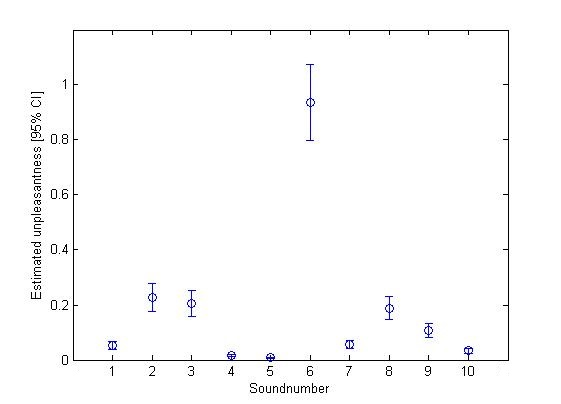
\includegraphics[width = 0.90\textwidth]{Figure/Confidens.jpg} 
\caption{Scale values and 95 \% confidence intervals}
\label{fig:Confidens}
\end{figure}